\documentclass[twoside]{book}

% Packages required by doxygen
\usepackage{fixltx2e}
\usepackage{calc}
\usepackage{doxygen}
\usepackage[export]{adjustbox} % also loads graphicx
\usepackage{graphicx}
\usepackage[utf8]{inputenc}
\usepackage{makeidx}
\usepackage{multicol}
\usepackage{multirow}
\PassOptionsToPackage{warn}{textcomp}
\usepackage{textcomp}
\usepackage[nointegrals]{wasysym}
\usepackage[table]{xcolor}

% Font selection
\usepackage[T1]{fontenc}
\usepackage[scaled=.90]{helvet}
\usepackage{courier}
\usepackage{amssymb}
\usepackage{sectsty}
\renewcommand{\familydefault}{\sfdefault}
\allsectionsfont{%
  \fontseries{bc}\selectfont%
  \color{darkgray}%
}
\renewcommand{\DoxyLabelFont}{%
  \fontseries{bc}\selectfont%
  \color{darkgray}%
}
\newcommand{\+}{\discretionary{\mbox{\scriptsize$\hookleftarrow$}}{}{}}

% Page & text layout
\usepackage{geometry}
\geometry{%
  a4paper,%
  top=2.5cm,%
  bottom=2.5cm,%
  left=2.5cm,%
  right=2.5cm%
}
\tolerance=750
\hfuzz=15pt
\hbadness=750
\setlength{\emergencystretch}{15pt}
\setlength{\parindent}{0cm}
\setlength{\parskip}{3ex plus 2ex minus 2ex}
\makeatletter
\renewcommand{\paragraph}{%
  \@startsection{paragraph}{4}{0ex}{-1.0ex}{1.0ex}{%
    \normalfont\normalsize\bfseries\SS@parafont%
  }%
}
\renewcommand{\subparagraph}{%
  \@startsection{subparagraph}{5}{0ex}{-1.0ex}{1.0ex}{%
    \normalfont\normalsize\bfseries\SS@subparafont%
  }%
}
\makeatother

% Headers & footers
\usepackage{fancyhdr}
\pagestyle{fancyplain}
\fancyhead[LE]{\fancyplain{}{\bfseries\thepage}}
\fancyhead[CE]{\fancyplain{}{}}
\fancyhead[RE]{\fancyplain{}{\bfseries\leftmark}}
\fancyhead[LO]{\fancyplain{}{\bfseries\rightmark}}
\fancyhead[CO]{\fancyplain{}{}}
\fancyhead[RO]{\fancyplain{}{\bfseries\thepage}}
\fancyfoot[LE]{\fancyplain{}{}}
\fancyfoot[CE]{\fancyplain{}{}}
\fancyfoot[RE]{\fancyplain{}{\bfseries\scriptsize Generated by Doxygen }}
\fancyfoot[LO]{\fancyplain{}{\bfseries\scriptsize Generated by Doxygen }}
\fancyfoot[CO]{\fancyplain{}{}}
\fancyfoot[RO]{\fancyplain{}{}}
\renewcommand{\footrulewidth}{0.4pt}
\renewcommand{\chaptermark}[1]{%
  \markboth{#1}{}%
}
\renewcommand{\sectionmark}[1]{%
  \markright{\thesection\ #1}%
}

% Indices & bibliography
\usepackage{natbib}
\usepackage[titles]{tocloft}
\setcounter{tocdepth}{3}
\setcounter{secnumdepth}{5}
\makeindex

% Hyperlinks (required, but should be loaded last)
\usepackage{ifpdf}
\ifpdf
  \usepackage[pdftex,pagebackref=true]{hyperref}
\else
  \usepackage[ps2pdf,pagebackref=true]{hyperref}
\fi
\hypersetup{%
  colorlinks=true,%
  linkcolor=blue,%
  citecolor=blue,%
  unicode%
}

% Custom commands
\newcommand{\clearemptydoublepage}{%
  \newpage{\pagestyle{empty}\cleardoublepage}%
}

\usepackage{caption}
\captionsetup{labelsep=space,justification=centering,font={bf},singlelinecheck=off,skip=4pt,position=top}

%===== C O N T E N T S =====

\begin{document}

% Titlepage & ToC
\hypersetup{pageanchor=false,
             bookmarksnumbered=true,
             pdfencoding=unicode
            }
\pagenumbering{roman}
\begin{titlepage}
\vspace*{7cm}
\begin{center}%
{\Large My Project }\\
\vspace*{1cm}
{\large Generated by Doxygen 1.8.11}\\
\end{center}
\end{titlepage}
\clearemptydoublepage
\tableofcontents
\clearemptydoublepage
\pagenumbering{arabic}
\hypersetup{pageanchor=true}

%--- Begin generated contents ---
\chapter{Robotic\+\_\+toy}
\label{md__home_viki_catkin_ws_src_Robotic_toy_README}
\hypertarget{md__home_viki_catkin_ws_src_Robotic_toy_README}{}
\href{https://github.com/Akshaybj0221/Robotic_toy/blob/master/LICENSE}{\tt } \href{https://travis-ci.org/Akshaybj0221/Robotic_toy}{\tt }

Robotic\+\_\+toy\+: A Robot Toy which moves in a polygon pattern as commanded by the user

This repository showcases the R\+OS package for the Robotic toy project. 



\subsection*{S\+IP Process\+:}

The S\+IP for the project can be found \href{https://docs.google.com/spreadsheets/d/1jLItNdomgrqtsU7UJ7i3CasUFsOEN9d-EHtjViunuMg/edit?usp=sharing}{\tt here}.

The Planning notes for the project can be found \href{https://docs.google.com/document/d/1cuM1NgHEFEkOeJMYtaNpIpAXfJ_u0YdG9ozSTAGEVLY/edit?usp=sharing}{\tt here}.

The link to the defect log, time log, product backlog, and release backlog table are as follows\+:

\href{https://docs.google.com/spreadsheets/d/1XhrbZjeozz02wAhwiE5d25f-5yS15jGHrX1-cPPEQfs/edit?usp=sharing}{\tt Product Backlog}.

\href{https://docs.google.com/spreadsheets/d/1TbC_kTvKK2MRH9XEX8YbNeR_NHrXO2tIK1uxxjgT04Y/edit?usp=sharing}{\tt Release Backlog Table}.

\href{https://docs.google.com/spreadsheets/d/1sQbnvWU1MZIwgt0YRekxqZq24jqrIhIC-pB-LOpDczo/edit?usp=sharing}{\tt Defect Log}

\subsection*{Dependencies/\+Prerequiesites}

The dependencies of this repository are\+:


\begin{DoxyCode}
1 * Ubuntu 16.04
2 * ROS Kinetic Kame
3 * TurtleBot
4 * Gazebo
\end{DoxyCode}


\subsection*{Building the code}

The code can be built by cloning the repository and executing following steps\+: 
\begin{DoxyCode}
1 <home>$ cd <workspace>/src
2 <workspace>/src$ git clone https://github.com/Akshaybj0221/Robotic\_toy.git
3 <workspace>/src$ cd ..
4 <workspace>$ catkin\_make 
\end{DoxyCode}


\subsection*{First sprint update}

Things done in the first sprint\+: \begin{DoxyVerb}* Install all the packages necessary to run Turtlebot in Gazebo and rviz
* Test the working of the necessary packages and check the data being received from the robot
* Explore various topics and packages that can be used in this project
* Create initial UML diagrams
* Setup Travis for the repository
* Create SIP log
\end{DoxyVerb}


\subsection*{Second sprint update}

Things done in second sprint\+: \begin{DoxyVerb}* Create a custom gazebo world that can be used a testing rig to test the performance of the algorithm 
* Create stub implementation of the class 
* Create Working test cases for the classes 
* Search how to input parameter in form of a service from user 
* Make a service for taking input from the user 
* Make a launch file to open Gazebo world, rviz and script  
* Control the Turtlebot using commandline as well as dummy script.
* Create planning notes and update SIP tasklog as well as release backlog. 
\end{DoxyVerb}


\subsection*{Results}

The software is very effective and fast in tracking any tagging motion simultaneously. Its funtionality has been tested on multiple test videos and software has a success rate of 98\%.

The working output of the software can be seen in the output folder of the repository or the link below\+: \href{https://github.com/Akshaybj0221/ENPM808X_Midterm.git}{\tt https\+://github.\+com/\+Akshaybj0221/\+E\+N\+P\+M808\+X\+\_\+\+Midterm.\+git}

\subsubsection*{Miscellaneous Instructions}


\begin{DoxyEnumerate}
\item cpplint and cppcheck output files are added in the {\itshape results} folder.
\item screenshots are added in the {\itshape output} folder.
\item {\itshape msg} folder is to be ignored as it has nothing relevant to the project.
\item {\itshape config} folder contains the custom log file. 
\end{DoxyEnumerate}
\chapter{Class Index}
\section{Class List}
Here are the classes, structs, unions and interfaces with brief descriptions\+:\begin{DoxyCompactList}
\item\contentsline{section}{\hyperlink{class_control_turtlebot}{Control\+Turtlebot} }{\pageref{class_control_turtlebot}}{}
\end{DoxyCompactList}

\chapter{File Index}
\section{File List}
Here is a list of all documented files with brief descriptions\+:\begin{DoxyCompactList}
\item\contentsline{section}{include/{\bfseries Control\+Turtlebot.\+hpp} }{\pageref{_control_turtlebot_8hpp}}{}
\item\contentsline{section}{src/\hyperlink{_control_turtlebot_8cpp}{Control\+Turtlebot.\+cpp} \\*Final Project -\/ Robotic Toy -\/ Moving in a polygonal trajectory inspired by users input }{\pageref{_control_turtlebot_8cpp}}{}
\item\contentsline{section}{src/\hyperlink{input_8cpp}{input.\+cpp} \\*Final Project -\/ Robotic Toy -\/ Moving in a polygonal trajectory inspired by users input }{\pageref{input_8cpp}}{}
\item\contentsline{section}{src/\hyperlink{main_8cpp}{main.\+cpp} \\*Final Project -\/ Robotic Toy -\/ Moving in a polygonal trajectory inspired by users input }{\pageref{main_8cpp}}{}
\item\contentsline{section}{test/{\bfseries test.\+cpp} }{\pageref{test_8cpp}}{}
\end{DoxyCompactList}

\chapter{Class Documentation}
\hypertarget{class_control_turtlebot}{}\section{Control\+Turtlebot Class Reference}
\label{class_control_turtlebot}\index{Control\+Turtlebot@{Control\+Turtlebot}}
\subsection*{Public Member Functions}
\begin{DoxyCompactItemize}
\item 
double \hyperlink{class_control_turtlebot_a000b59ff871ccee120ea9ad36a24922a}{circle} (double speed)
\begin{DoxyCompactList}\small\item\em Take the action. \end{DoxyCompactList}\item 
void \hyperlink{class_control_turtlebot_abca7a1b114375081608e8e17edebaf22}{pose\+Callback} (const nav\+\_\+msgs\+::\+Odometry\+::\+Const\+Ptr \&pose\+\_\+message)
\begin{DoxyCompactList}\small\item\em Callback function for service. \end{DoxyCompactList}\item 
void \hyperlink{class_control_turtlebot_a71259921f0318cea8ce13838eef9402e}{move\+\_\+linear} (double speed, double distance, bool is\+Forward, double total\+Sides)
\begin{DoxyCompactList}\small\item\em linearly moving funtion/method \end{DoxyCompactList}\item 
double \hyperlink{class_control_turtlebot_a0c5c4a568758d3165e7f275d0f666afb}{rotate} (double ang\+\_\+vel, double angle\+\_\+radian, bool is\+Clockwise)
\begin{DoxyCompactList}\small\item\em Executes the rotation for turtlebot. \end{DoxyCompactList}\item 
double \hyperlink{class_control_turtlebot_adcb5d2af5d989a8f2088ff13136bfc1a}{degree2radian} (double degree\+Angle)
\begin{DoxyCompactList}\small\item\em makes conversion from degree to degree \end{DoxyCompactList}\item 
double \hyperlink{class_control_turtlebot_ac20a23af7bd0978dd47b9dc5a0e0b880}{radian2degree} (double radian\+Angle)
\begin{DoxyCompactList}\small\item\em makes conversion from radian to degree \end{DoxyCompactList}\item 
void \hyperlink{class_control_turtlebot_ac23a9389982e796ddb302ea158d370d6}{move\+Shape} (double side\+Length, double total\+Sides, double angle, double velocity)
\begin{DoxyCompactList}\small\item\em Executes the planned trajectory for turtlebot. \end{DoxyCompactList}\end{DoxyCompactItemize}
\subsection*{Public Attributes}
\begin{DoxyCompactItemize}
\item 
ros\+::\+Publisher {\bfseries pub}\hypertarget{class_control_turtlebot_a9334d4337499cdde728423b9e2c95152}{}\label{class_control_turtlebot_a9334d4337499cdde728423b9e2c95152}

\item 
ros\+::\+Subscriber {\bfseries pose\+\_\+subscriber}\hypertarget{class_control_turtlebot_a3f70b9134199b02477917d404c6046ce}{}\label{class_control_turtlebot_a3f70b9134199b02477917d404c6046ce}

\item 
nav\+\_\+msgs\+::\+Odometry {\bfseries turtlebot\+\_\+odom\+\_\+pose}\hypertarget{class_control_turtlebot_a34fe24732253b38c4eaead6d9ecc0405}{}\label{class_control_turtlebot_a34fe24732253b38c4eaead6d9ecc0405}

\item 
ros\+::\+Node\+Handle {\bfseries n}\hypertarget{class_control_turtlebot_a7aba89f4135d80c5973fe6e923f56176}{}\label{class_control_turtlebot_a7aba89f4135d80c5973fe6e923f56176}

\end{DoxyCompactItemize}


\subsection{Detailed Description}


Definition at line 52 of file Control\+Turtlebot.\+hpp.



\subsection{Member Function Documentation}
\index{Control\+Turtlebot@{Control\+Turtlebot}!circle@{circle}}
\index{circle@{circle}!Control\+Turtlebot@{Control\+Turtlebot}}
\subsubsection[{\texorpdfstring{circle(double speed)}{circle(double speed)}}]{\setlength{\rightskip}{0pt plus 5cm}double Control\+Turtlebot\+::circle (
\begin{DoxyParamCaption}
\item[{double}]{speed}
\end{DoxyParamCaption}
)}\hypertarget{class_control_turtlebot_a000b59ff871ccee120ea9ad36a24922a}{}\label{class_control_turtlebot_a000b59ff871ccee120ea9ad36a24922a}


Take the action. 

Executes a dummy trajectory for turtlebot.

Move robot in a random dummy trajectory \begin{DoxyReturn}{Returns}
double\+: Return true
\end{DoxyReturn}

\begin{DoxyParams}[1]{Parameters}
\mbox{\tt in}  & {\em velocity} & Velocity of robot \\
\hline
\end{DoxyParams}


Definition at line 134 of file Control\+Turtlebot.\+cpp.

\index{Control\+Turtlebot@{Control\+Turtlebot}!degree2radian@{degree2radian}}
\index{degree2radian@{degree2radian}!Control\+Turtlebot@{Control\+Turtlebot}}
\subsubsection[{\texorpdfstring{degree2radian(double degree\+Angle)}{degree2radian(double degreeAngle)}}]{\setlength{\rightskip}{0pt plus 5cm}double Control\+Turtlebot\+::degree2radian (
\begin{DoxyParamCaption}
\item[{double}]{degree\+Angle}
\end{DoxyParamCaption}
)}\hypertarget{class_control_turtlebot_adcb5d2af5d989a8f2088ff13136bfc1a}{}\label{class_control_turtlebot_adcb5d2af5d989a8f2088ff13136bfc1a}


makes conversion from degree to degree 

makes conversion from degree to radian


\begin{DoxyParams}[1]{Parameters}
\mbox{\tt in}  & {\em radian\+Angle} & Angle by which the robot needs to turn\\
\hline
\end{DoxyParams}
\begin{DoxyReturn}{Returns}
bool\+: Return true if succeeded
\end{DoxyReturn}

\begin{DoxyParams}[1]{Parameters}
\mbox{\tt in}  & {\em radian\+Angle} & Angle by which the robot needs to turn \\
\hline
\end{DoxyParams}


Definition at line 261 of file Control\+Turtlebot.\+cpp.

\index{Control\+Turtlebot@{Control\+Turtlebot}!move\+\_\+linear@{move\+\_\+linear}}
\index{move\+\_\+linear@{move\+\_\+linear}!Control\+Turtlebot@{Control\+Turtlebot}}
\subsubsection[{\texorpdfstring{move\+\_\+linear(double speed, double distance, bool is\+Forward, double total\+Sides)}{move_linear(double speed, double distance, bool isForward, double totalSides)}}]{\setlength{\rightskip}{0pt plus 5cm}void Control\+Turtlebot\+::move\+\_\+linear (
\begin{DoxyParamCaption}
\item[{double}]{speed, }
\item[{double}]{distance, }
\item[{bool}]{is\+Forward, }
\item[{double}]{total\+Sides}
\end{DoxyParamCaption}
)}\hypertarget{class_control_turtlebot_a71259921f0318cea8ce13838eef9402e}{}\label{class_control_turtlebot_a71259921f0318cea8ce13838eef9402e}


linearly moving funtion/method 

Makes the turtlebot move in a straight line at a particular distance.

the function that makes the robot moves forward and backward


\begin{DoxyParams}{Parameters}
{\em distance} & Length of one side of the polygonal trajectory \\
\hline
{\em total\+Sides} & Total number of sides inserted by the user \\
\hline
{\em is\+Forward} & To check if forward moving value or backward \\
\hline
{\em speed} & Velocity of robot\\
\hline
\end{DoxyParams}
\begin{DoxyReturn}{Returns}
bool\+: Return true if succeeded
\end{DoxyReturn}

\begin{DoxyParams}[1]{Parameters}
\mbox{\tt in}  & {\em distance} & Length of one side of the polygonal trajectory \\
\hline
\mbox{\tt in}  & {\em total\+Sides} & Total number of sides inserted by the user \\
\hline
\mbox{\tt in}  & {\em speed} & Velocity of robot \\
\hline
 & {\em is\+Forward} & To check if forward moving value or backward \\
\hline
\end{DoxyParams}


Definition at line 88 of file Control\+Turtlebot.\+cpp.

\index{Control\+Turtlebot@{Control\+Turtlebot}!move\+Shape@{move\+Shape}}
\index{move\+Shape@{move\+Shape}!Control\+Turtlebot@{Control\+Turtlebot}}
\subsubsection[{\texorpdfstring{move\+Shape(double side\+Length, double total\+Sides, double angle, double velocity)}{moveShape(double sideLength, double totalSides, double angle, double velocity)}}]{\setlength{\rightskip}{0pt plus 5cm}void Control\+Turtlebot\+::move\+Shape (
\begin{DoxyParamCaption}
\item[{double}]{side\+Length, }
\item[{double}]{total\+Sides, }
\item[{double}]{angle, }
\item[{double}]{velocity}
\end{DoxyParamCaption}
)}\hypertarget{class_control_turtlebot_ac23a9389982e796ddb302ea158d370d6}{}\label{class_control_turtlebot_ac23a9389982e796ddb302ea158d370d6}


Executes the planned trajectory for turtlebot. 


\begin{DoxyParams}[1]{Parameters}
\mbox{\tt in}  & {\em side\+Length} & Length of one side of the polygonal trajectory \\
\hline
\mbox{\tt in}  & {\em total\+Sides} & Total number of sides inserted by the user \\
\hline
\mbox{\tt in}  & {\em angle} & Angle by which the robot needs to turn \\
\hline
\mbox{\tt in}  & {\em velocity} & Velocity of robot\\
\hline
\end{DoxyParams}
\begin{DoxyReturn}{Returns}
void\+: Return nothing
\end{DoxyReturn}

\begin{DoxyParams}[1]{Parameters}
\mbox{\tt in}  & {\em side\+Length} & Length of one side of the polygonal trajectory \\
\hline
\mbox{\tt in}  & {\em total\+Sides} & Total number of sides inserted by the user \\
\hline
\mbox{\tt in}  & {\em angle} & Angle by which the robot needs to turn \\
\hline
\mbox{\tt in}  & {\em velocity} & Velocity of robot \\
\hline
\end{DoxyParams}


Definition at line 65 of file Control\+Turtlebot.\+cpp.

\index{Control\+Turtlebot@{Control\+Turtlebot}!pose\+Callback@{pose\+Callback}}
\index{pose\+Callback@{pose\+Callback}!Control\+Turtlebot@{Control\+Turtlebot}}
\subsubsection[{\texorpdfstring{pose\+Callback(const nav\+\_\+msgs\+::\+Odometry\+::\+Const\+Ptr \&pose\+\_\+message)}{poseCallback(const nav_msgs::Odometry::ConstPtr &pose_message)}}]{\setlength{\rightskip}{0pt plus 5cm}void Control\+Turtlebot\+::pose\+Callback (
\begin{DoxyParamCaption}
\item[{const nav\+\_\+msgs\+::\+Odometry\+::\+Const\+Ptr \&}]{pose\+\_\+message}
\end{DoxyParamCaption}
)}\hypertarget{class_control_turtlebot_abca7a1b114375081608e8e17edebaf22}{}\label{class_control_turtlebot_abca7a1b114375081608e8e17edebaf22}


Callback function for service. 

Callback for the Odometry data.

Function callback for the service input


\begin{DoxyParams}{Parameters}
{\em pose\+\_\+message} & Service message\\
\hline
\end{DoxyParams}
\begin{DoxyReturn}{Returns}
void\+: Return nothing
\end{DoxyReturn}

\begin{DoxyParams}[1]{Parameters}
\mbox{\tt in}  & {\em pose\+\_\+message} & The message \\
\hline
\end{DoxyParams}


Definition at line 42 of file Control\+Turtlebot.\+cpp.

\index{Control\+Turtlebot@{Control\+Turtlebot}!radian2degree@{radian2degree}}
\index{radian2degree@{radian2degree}!Control\+Turtlebot@{Control\+Turtlebot}}
\subsubsection[{\texorpdfstring{radian2degree(double radian\+Angle)}{radian2degree(double radianAngle)}}]{\setlength{\rightskip}{0pt plus 5cm}double Control\+Turtlebot\+::radian2degree (
\begin{DoxyParamCaption}
\item[{double}]{radian\+Angle}
\end{DoxyParamCaption}
)}\hypertarget{class_control_turtlebot_ac20a23af7bd0978dd47b9dc5a0e0b880}{}\label{class_control_turtlebot_ac20a23af7bd0978dd47b9dc5a0e0b880}


makes conversion from radian to degree 


\begin{DoxyParams}[1]{Parameters}
\mbox{\tt in}  & {\em radian\+Angle} & Angle by which the robot needs to turn\\
\hline
\end{DoxyParams}
\begin{DoxyReturn}{Returns}
bool\+: Return true if succeeded
\end{DoxyReturn}

\begin{DoxyParams}[1]{Parameters}
\mbox{\tt in}  & {\em radian\+Angle} & Angle by which the robot needs to turn \\
\hline
\end{DoxyParams}


Definition at line 251 of file Control\+Turtlebot.\+cpp.

\index{Control\+Turtlebot@{Control\+Turtlebot}!rotate@{rotate}}
\index{rotate@{rotate}!Control\+Turtlebot@{Control\+Turtlebot}}
\subsubsection[{\texorpdfstring{rotate(double ang\+\_\+vel, double angle\+\_\+radian, bool is\+Clockwise)}{rotate(double ang_vel, double angle_radian, bool isClockwise)}}]{\setlength{\rightskip}{0pt plus 5cm}double Control\+Turtlebot\+::rotate (
\begin{DoxyParamCaption}
\item[{double}]{angular\+\_\+velocity, }
\item[{double}]{radians, }
\item[{bool}]{clockwise}
\end{DoxyParamCaption}
)}\hypertarget{class_control_turtlebot_a0c5c4a568758d3165e7f275d0f666afb}{}\label{class_control_turtlebot_a0c5c4a568758d3165e7f275d0f666afb}


Executes the rotation for turtlebot. 

the function that makes the robot rotate


\begin{DoxyParams}[1]{Parameters}
\mbox{\tt in}  & {\em is\+Clockwise} & To make sure robot always rotates in a clockwise direction \\
\hline
\mbox{\tt in}  & {\em angle\+\_\+radian} & Angle by which the robot needs to turn \\
\hline
\mbox{\tt in}  & {\em angular\+\_\+vel} & Velocity of robot rotation\\
\hline
\end{DoxyParams}
\begin{DoxyReturn}{Returns}
bool\+: Return true if succeeded
\end{DoxyReturn}

\begin{DoxyParams}[1]{Parameters}
\mbox{\tt in}  & {\em clockwise} & To make sure robot always rotates in a clockwise direction \\
\hline
\mbox{\tt in}  & {\em radians} & Angle by which the robot needs to turn \\
\hline
\mbox{\tt in}  & {\em angular\+\_\+velocity} & Velocity of robot rotation \\
\hline
\end{DoxyParams}


Definition at line 150 of file Control\+Turtlebot.\+cpp.



The documentation for this class was generated from the following files\+:\begin{DoxyCompactItemize}
\item 
include/Control\+Turtlebot.\+hpp\item 
src/\hyperlink{_control_turtlebot_8cpp}{Control\+Turtlebot.\+cpp}\end{DoxyCompactItemize}

\chapter{File Documentation}
\hypertarget{_control_turtlebot_8cpp}{}\section{/home/viki/catkin\+\_\+ws/src/\+Robotic\+\_\+toy/src/\+Control\+Turtlebot.cpp File Reference}
\label{_control_turtlebot_8cpp}\index{/home/viki/catkin\+\_\+ws/src/\+Robotic\+\_\+toy/src/\+Control\+Turtlebot.\+cpp@{/home/viki/catkin\+\_\+ws/src/\+Robotic\+\_\+toy/src/\+Control\+Turtlebot.\+cpp}}


Final Project -\/ Robotic Toy -\/ Moving in a polygonal trajectory inspired by users input.  


{\ttfamily \#include \char`\"{}Control\+Turtlebot.\+hpp\char`\"{}}\\*
Include dependency graph for Control\+Turtlebot.\+cpp\+:
\nopagebreak
\begin{figure}[H]
\begin{center}
\leavevmode
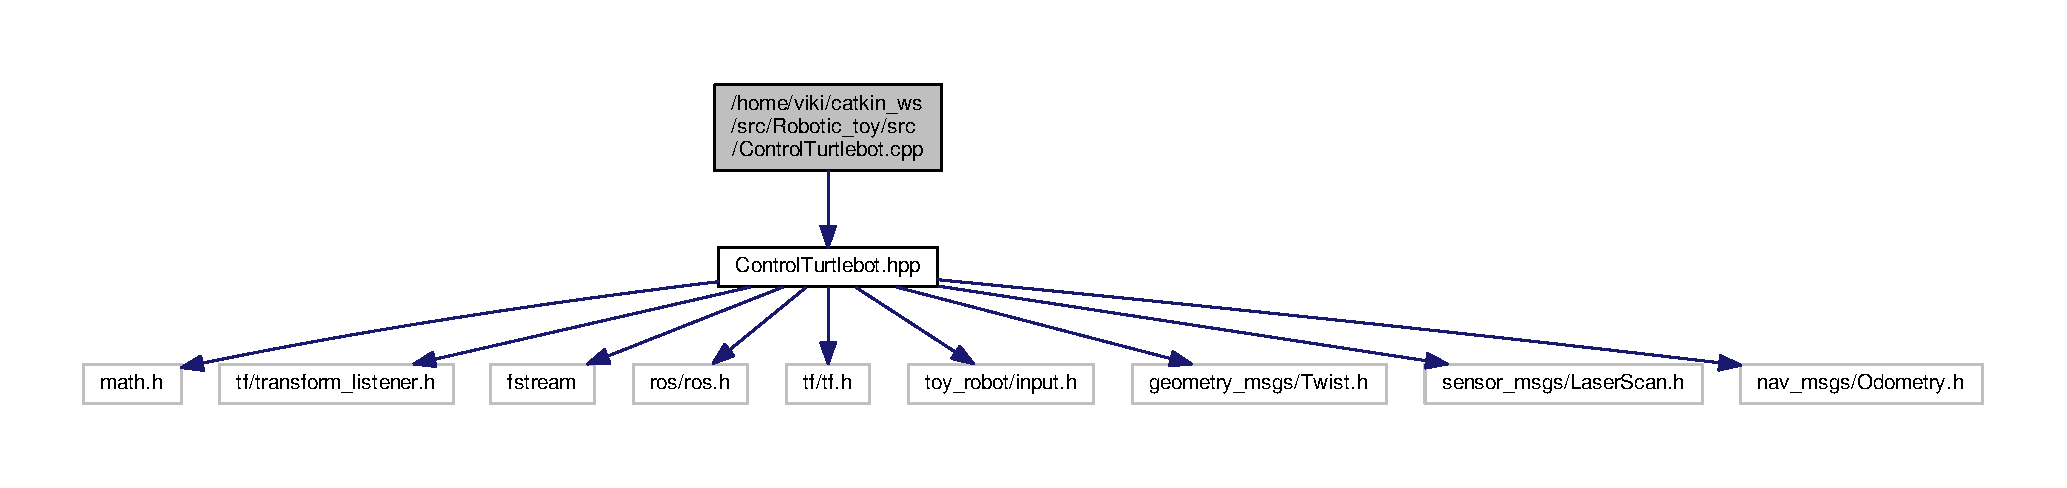
\includegraphics[width=350pt]{_control_turtlebot_8cpp__incl}
\end{center}
\end{figure}


\subsection{Detailed Description}
Final Project -\/ Robotic Toy -\/ Moving in a polygonal trajectory inspired by users input. 

M\+IT License

Copyright (c) 2017 Karan Vivek Bhargava

Permission is hereby granted, free of charge, to any person obtaining a copy of this software and associated documentation files (the \char`\"{}\+Software\char`\"{}), to deal in the Software without restriction, including without limitation the rights to use, copy, modify, merge, publish, distribute, sublicense, and/or sell copies of the Software, and to permit persons to whom the Software is furnished to do so, subject to the following conditions\+:

The above copyright notice and this permission notice shall be included in all copies or substantial portions of the Software.

T\+HE S\+O\+F\+T\+W\+A\+RE IS P\+R\+O\+V\+I\+D\+ED \char`\"{}\+A\+S I\+S\char`\"{}, W\+I\+T\+H\+O\+UT W\+A\+R\+R\+A\+N\+TY OF A\+NY K\+I\+ND, E\+X\+P\+R\+E\+SS OR I\+M\+P\+L\+I\+ED, I\+N\+C\+L\+U\+D\+I\+NG B\+UT N\+OT L\+I\+M\+I\+T\+ED TO T\+HE W\+A\+R\+R\+A\+N\+T\+I\+ES OF M\+E\+R\+C\+H\+A\+N\+T\+A\+B\+I\+L\+I\+TY, F\+I\+T\+N\+E\+SS F\+OR A P\+A\+R\+T\+I\+C\+U\+L\+AR P\+U\+R\+P\+O\+SE A\+ND N\+O\+N\+I\+N\+F\+R\+I\+N\+G\+E\+M\+E\+NT. IN NO E\+V\+E\+NT S\+H\+A\+LL T\+HE A\+U\+T\+H\+O\+RS OR C\+O\+P\+Y\+R\+I\+G\+HT H\+O\+L\+D\+E\+RS BE L\+I\+A\+B\+LE F\+OR A\+NY C\+L\+A\+IM, D\+A\+M\+A\+G\+ES OR O\+T\+H\+ER L\+I\+A\+B\+I\+L\+I\+TY, W\+H\+E\+T\+H\+ER IN AN A\+C\+T\+I\+ON OF C\+O\+N\+T\+R\+A\+CT, T\+O\+RT OR O\+T\+H\+E\+R\+W\+I\+SE, A\+R\+I\+S\+I\+NG F\+R\+OM, O\+UT OF OR IN C\+O\+N\+N\+E\+C\+T\+I\+ON W\+I\+TH T\+HE S\+O\+F\+T\+W\+A\+RE OR T\+HE U\+SE OR O\+T\+H\+ER D\+E\+A\+L\+I\+N\+GS IN T\+HE S\+O\+F\+T\+W\+A\+RE.

\begin{DoxyAuthor}{Author}
Akshay Bajaj 
\end{DoxyAuthor}
\begin{DoxyCopyright}{Copyright}
M\+IT License (c) 2017 Akshay Bajaj
\end{DoxyCopyright}
\hypertarget{main_8cpp_DESCRIPTION}{}\subsection{D\+E\+S\+C\+R\+I\+P\+T\+I\+ON}\label{main_8cpp_DESCRIPTION}
This program will instantiate a input server node, and service server \char`\"{}input\char`\"{} 
\hypertarget{input_8cpp}{}\section{src/input.cpp File Reference}
\label{input_8cpp}\index{src/input.\+cpp@{src/input.\+cpp}}


Final Project -\/ Robotic Toy -\/ Moving in a polygonal trajectory inspired by users input.  


{\ttfamily \#include $<$cstdlib$>$}\\*
{\ttfamily \#include \char`\"{}ros/ros.\+h\char`\"{}}\\*
{\ttfamily \#include \char`\"{}toy\+\_\+robot/input.\+h\char`\"{}}\\*
Include dependency graph for input.\+cpp\+:\nopagebreak
\begin{figure}[H]
\begin{center}
\leavevmode
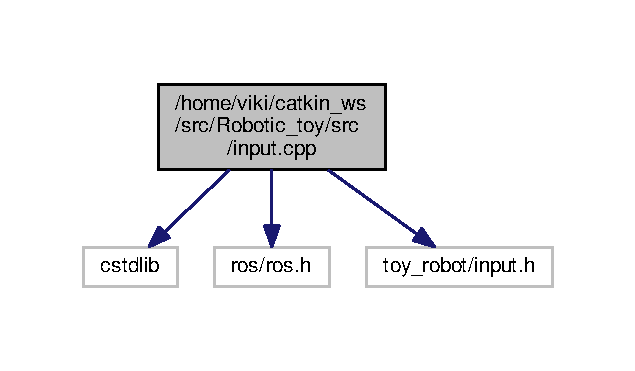
\includegraphics[width=305pt]{input_8cpp__incl}
\end{center}
\end{figure}
\subsection*{Functions}
\begin{DoxyCompactItemize}
\item 
bool {\bfseries add} (toy\+\_\+robot\+::input\+::\+Request \&req, toy\+\_\+robot\+::input\+::\+Response \&res)\hypertarget{input_8cpp_aa84412adb178b06ce9679b3db460087a}{}\label{input_8cpp_aa84412adb178b06ce9679b3db460087a}

\item 
int {\bfseries main} (int argc, char $\ast$$\ast$argv)\hypertarget{input_8cpp_a3c04138a5bfe5d72780bb7e82a18e627}{}\label{input_8cpp_a3c04138a5bfe5d72780bb7e82a18e627}

\end{DoxyCompactItemize}


\subsection{Detailed Description}
Final Project -\/ Robotic Toy -\/ Moving in a polygonal trajectory inspired by users input. 

M\+IT License

Copyright (c) 2017 Karan Vivek Bhargava

Permission is hereby granted, free of charge, to any person obtaining a copy of this software and associated documentation files (the \char`\"{}\+Software\char`\"{}), to deal in the Software without restriction, including without limitation the rights to use, copy, modify, merge, publish, distribute, sublicense, and/or sell copies of the Software, and to permit persons to whom the Software is furnished to do so, subject to the following conditions\+:

The above copyright notice and this permission notice shall be included in all copies or substantial portions of the Software.

T\+HE S\+O\+F\+T\+W\+A\+RE IS P\+R\+O\+V\+I\+D\+ED \char`\"{}\+A\+S I\+S\char`\"{}, W\+I\+T\+H\+O\+UT W\+A\+R\+R\+A\+N\+TY OF A\+NY K\+I\+ND, E\+X\+P\+R\+E\+SS OR I\+M\+P\+L\+I\+ED, I\+N\+C\+L\+U\+D\+I\+NG B\+UT N\+OT L\+I\+M\+I\+T\+ED TO T\+HE W\+A\+R\+R\+A\+N\+T\+I\+ES OF M\+E\+R\+C\+H\+A\+N\+T\+A\+B\+I\+L\+I\+TY, F\+I\+T\+N\+E\+SS F\+OR A P\+A\+R\+T\+I\+C\+U\+L\+AR P\+U\+R\+P\+O\+SE A\+ND N\+O\+N\+I\+N\+F\+R\+I\+N\+G\+E\+M\+E\+NT. IN NO E\+V\+E\+NT S\+H\+A\+LL T\+HE A\+U\+T\+H\+O\+RS OR C\+O\+P\+Y\+R\+I\+G\+HT H\+O\+L\+D\+E\+RS BE L\+I\+A\+B\+LE F\+OR A\+NY C\+L\+A\+IM, D\+A\+M\+A\+G\+ES OR O\+T\+H\+ER L\+I\+A\+B\+I\+L\+I\+TY, W\+H\+E\+T\+H\+ER IN AN A\+C\+T\+I\+ON OF C\+O\+N\+T\+R\+A\+CT, T\+O\+RT OR O\+T\+H\+E\+R\+W\+I\+SE, A\+R\+I\+S\+I\+NG F\+R\+OM, O\+UT OF OR IN C\+O\+N\+N\+E\+C\+T\+I\+ON W\+I\+TH T\+HE S\+O\+F\+T\+W\+A\+RE OR T\+HE U\+SE OR O\+T\+H\+ER D\+E\+A\+L\+I\+N\+GS IN T\+HE S\+O\+F\+T\+W\+A\+RE.

\begin{DoxyAuthor}{Author}
Akshay Bajaj 
\end{DoxyAuthor}
\begin{DoxyCopyright}{Copyright}
M\+IT License (c) 2017 Akshay Bajaj
\end{DoxyCopyright}
\hypertarget{main_8cpp_DESCRIPTION}{}\subsection{D\+E\+S\+C\+R\+I\+P\+T\+I\+ON}\label{main_8cpp_DESCRIPTION}
This program will instantiate a input server node, and service server \char`\"{}input\char`\"{} 
\hypertarget{main_8cpp}{}\section{/home/viki/catkin\+\_\+ws/src/\+Robotic\+\_\+toy/src/main.cpp File Reference}
\label{main_8cpp}\index{/home/viki/catkin\+\_\+ws/src/\+Robotic\+\_\+toy/src/main.\+cpp@{/home/viki/catkin\+\_\+ws/src/\+Robotic\+\_\+toy/src/main.\+cpp}}


Final Project -\/ Robotic Toy -\/ Moving in a polygonal trajectory inspired by users input.  


{\ttfamily \#include \char`\"{}Control\+Turtlebot.\+hpp\char`\"{}}\\*
Include dependency graph for main.\+cpp\+:
\nopagebreak
\begin{figure}[H]
\begin{center}
\leavevmode
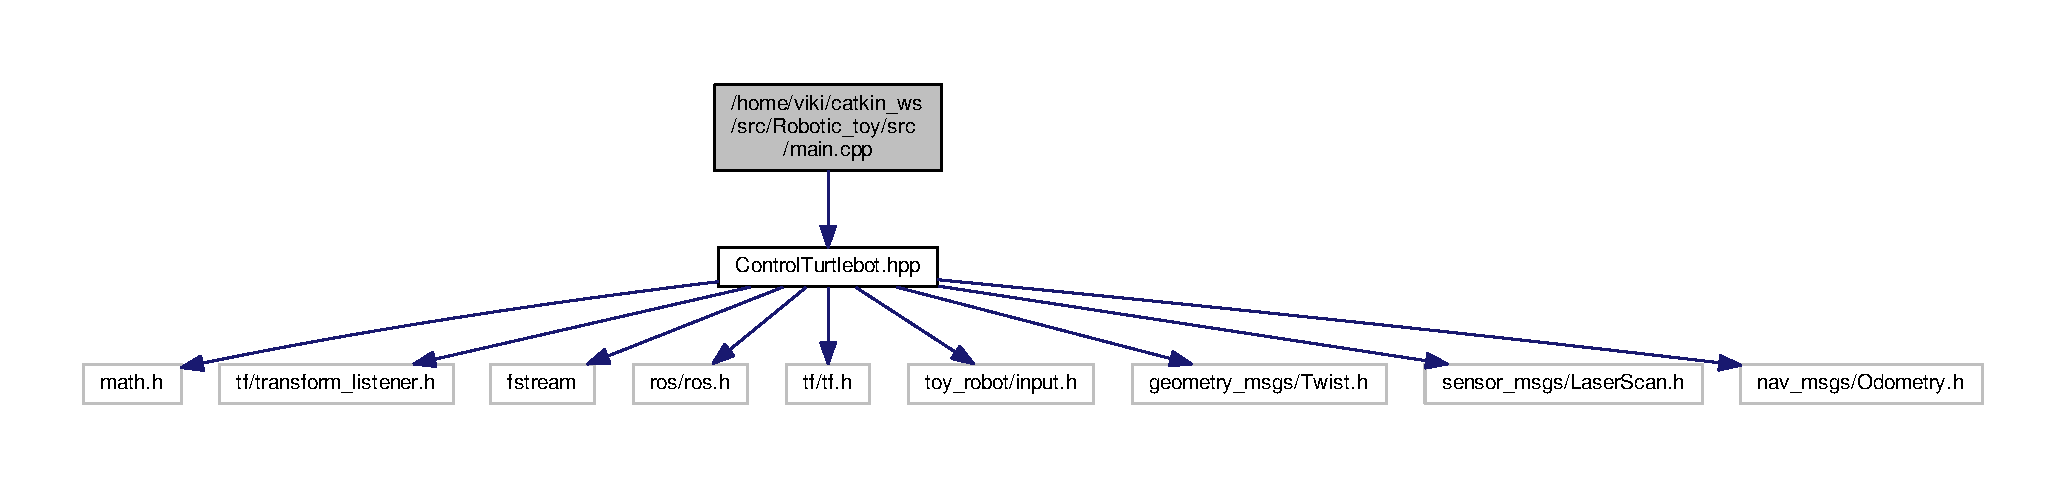
\includegraphics[width=350pt]{main_8cpp__incl}
\end{center}
\end{figure}
\subsection*{Functions}
\begin{DoxyCompactItemize}
\item 
int {\bfseries main} (int argc, char $\ast$$\ast$argv)\hypertarget{main_8cpp_a3c04138a5bfe5d72780bb7e82a18e627}{}\label{main_8cpp_a3c04138a5bfe5d72780bb7e82a18e627}

\end{DoxyCompactItemize}


\subsection{Detailed Description}
Final Project -\/ Robotic Toy -\/ Moving in a polygonal trajectory inspired by users input. 

M\+IT License

Copyright (c) 2017 Karan Vivek Bhargava

Permission is hereby granted, free of charge, to any person obtaining a copy of this software and associated documentation files (the \char`\"{}\+Software\char`\"{}), to deal in the Software without restriction, including without limitation the rights to use, copy, modify, merge, publish, distribute, sublicense, and/or sell copies of the Software, and to permit persons to whom the Software is furnished to do so, subject to the following conditions\+:

The above copyright notice and this permission notice shall be included in all copies or substantial portions of the Software.

T\+HE S\+O\+F\+T\+W\+A\+RE IS P\+R\+O\+V\+I\+D\+ED \char`\"{}\+A\+S I\+S\char`\"{}, W\+I\+T\+H\+O\+UT W\+A\+R\+R\+A\+N\+TY OF A\+NY K\+I\+ND, E\+X\+P\+R\+E\+SS OR I\+M\+P\+L\+I\+ED, I\+N\+C\+L\+U\+D\+I\+NG B\+UT N\+OT L\+I\+M\+I\+T\+ED TO T\+HE W\+A\+R\+R\+A\+N\+T\+I\+ES OF M\+E\+R\+C\+H\+A\+N\+T\+A\+B\+I\+L\+I\+TY, F\+I\+T\+N\+E\+SS F\+OR A P\+A\+R\+T\+I\+C\+U\+L\+AR P\+U\+R\+P\+O\+SE A\+ND N\+O\+N\+I\+N\+F\+R\+I\+N\+G\+E\+M\+E\+NT. IN NO E\+V\+E\+NT S\+H\+A\+LL T\+HE A\+U\+T\+H\+O\+RS OR C\+O\+P\+Y\+R\+I\+G\+HT H\+O\+L\+D\+E\+RS BE L\+I\+A\+B\+LE F\+OR A\+NY C\+L\+A\+IM, D\+A\+M\+A\+G\+ES OR O\+T\+H\+ER L\+I\+A\+B\+I\+L\+I\+TY, W\+H\+E\+T\+H\+ER IN AN A\+C\+T\+I\+ON OF C\+O\+N\+T\+R\+A\+CT, T\+O\+RT OR O\+T\+H\+E\+R\+W\+I\+SE, A\+R\+I\+S\+I\+NG F\+R\+OM, O\+UT OF OR IN C\+O\+N\+N\+E\+C\+T\+I\+ON W\+I\+TH T\+HE S\+O\+F\+T\+W\+A\+RE OR T\+HE U\+SE OR O\+T\+H\+ER D\+E\+A\+L\+I\+N\+GS IN T\+HE S\+O\+F\+T\+W\+A\+RE.

\begin{DoxyAuthor}{Author}
Akshay Bajaj 
\end{DoxyAuthor}
\begin{DoxyCopyright}{Copyright}
M\+IT License (c) 2017 Akshay Bajaj
\end{DoxyCopyright}
\hypertarget{main_8cpp_DESCRIPTION}{}\subsection{D\+E\+S\+C\+R\+I\+P\+T\+I\+ON}\label{main_8cpp_DESCRIPTION}
This program will instantiate a free space navigation node, and service client \char`\"{}input\char`\"{} 
%--- End generated contents ---

% Index
\backmatter
\newpage
\phantomsection
\clearemptydoublepage
\addcontentsline{toc}{chapter}{Index}
\printindex

\end{document}
